\documentclass{scrartcl}
\usepackage[a4paper,left=1in,right=1in,top=1.2in,bottom=1in]{geometry}
\usepackage{siunitx}
\usepackage{graphicx}
\usepackage{mathtools}
\setkomafont{disposition}{\normalfont\bfseries}
\newcommand*\diff{\mathop{}\!\mathrm{d}}
\newcommand*\Diff[1]{\mathop{}\!\mathrm{d^#1}}
\newcommand*\colvec[3][]{
    \begin{pmatrix}\ifx\relax#1\relax\else#1\\\fi#2\\#3\end{pmatrix}
}

%title
\title{Exercise 07:\\Expectation maximization}
\subtitle{Theoretical Neuroscience II}
\author{Johannes G\"atjen \and Lorena Morton}

%use these for structure/overview
\newcommand\Question{%
  \textbf{Question:}%
}
\newcommand\Answer{%
  \textbf{Answer:}%
}
\renewcommand{\arraystretch}{1.2}


\begin{document}
\maketitle


\begin{figure}[h]
\centering
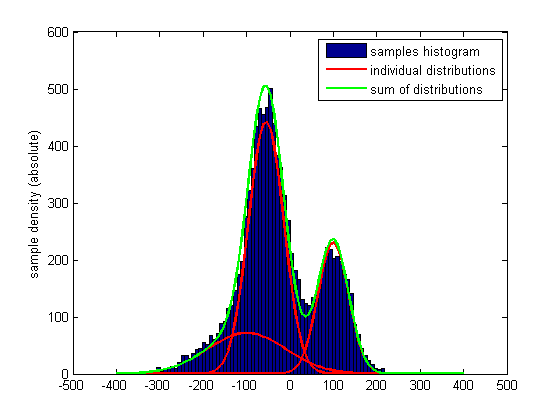
\includegraphics[trim = {0.7cm 0.5cm 1cm 0.7cm}, width=0.8\textwidth, clip]{../pics/manual}
\caption{Histogram of original samples and manually estimated underlying distributions.}
\label{}
\end{figure}

\begin{figure}[h]
\centering
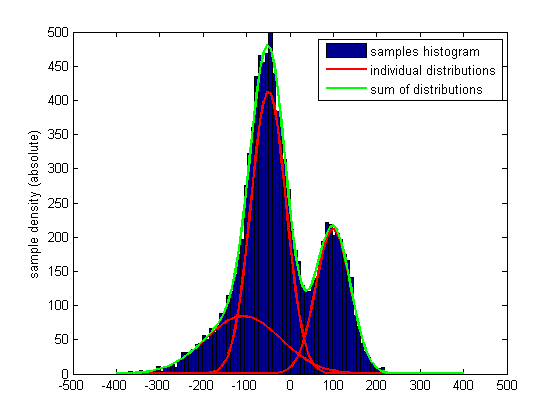
\includegraphics[trim = {0.7cm 0.5cm 1cm 0.7cm}, width=0.8\textwidth, clip]{../pics/em}
\caption{Histogram of original samples and underlying distributions estimated with expectation maximization.}
\label{}
\end{figure}

\end{document}